The Sumeru Desert is home to many mountains, most of which are unclimbable, causing inconvenience for travelers.

As is widely known, Venti from Mondstadt once leveled Mondstadt's mountainous terrain by submerging the mountain ranges into the sea, giving rise to the Golden Apple Archipelago.

However, Venti can't level these mountains, but he can assist you in ascending them \textbf{at most once}.

These mountains can be roughly considered as polygons, as depicted in the diagram below, where the vertices of the shortest path must reside on the vertices of the obstacle polygons.

\begin{center}
    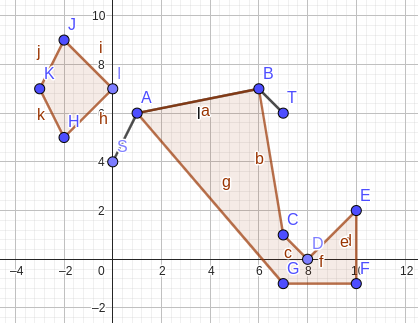
\includegraphics[scale=0.8]{example.png} \\
    \small{The shortest path from $S$ to $T$}
\end{center}

Considering this problem might be too challenging for you, Venti has taken care of the geometric relationships. Specifically, he will provide you with information on the starting point, ending point, pairs of points between vertices of each polygon that are reachable without climbing, exactly once reachable pairs with a climb, and the distances between these pairs.

If you find it hard to grasp, don't worry. In formal terms, you are given an undirected weighted graph with edges in two colors (red and blue). Your task is to find the shortest path from the starting point to the ending point, passing through at most one blue edge, or confirm that reaching the ending point is impossible.

\begin{center}
    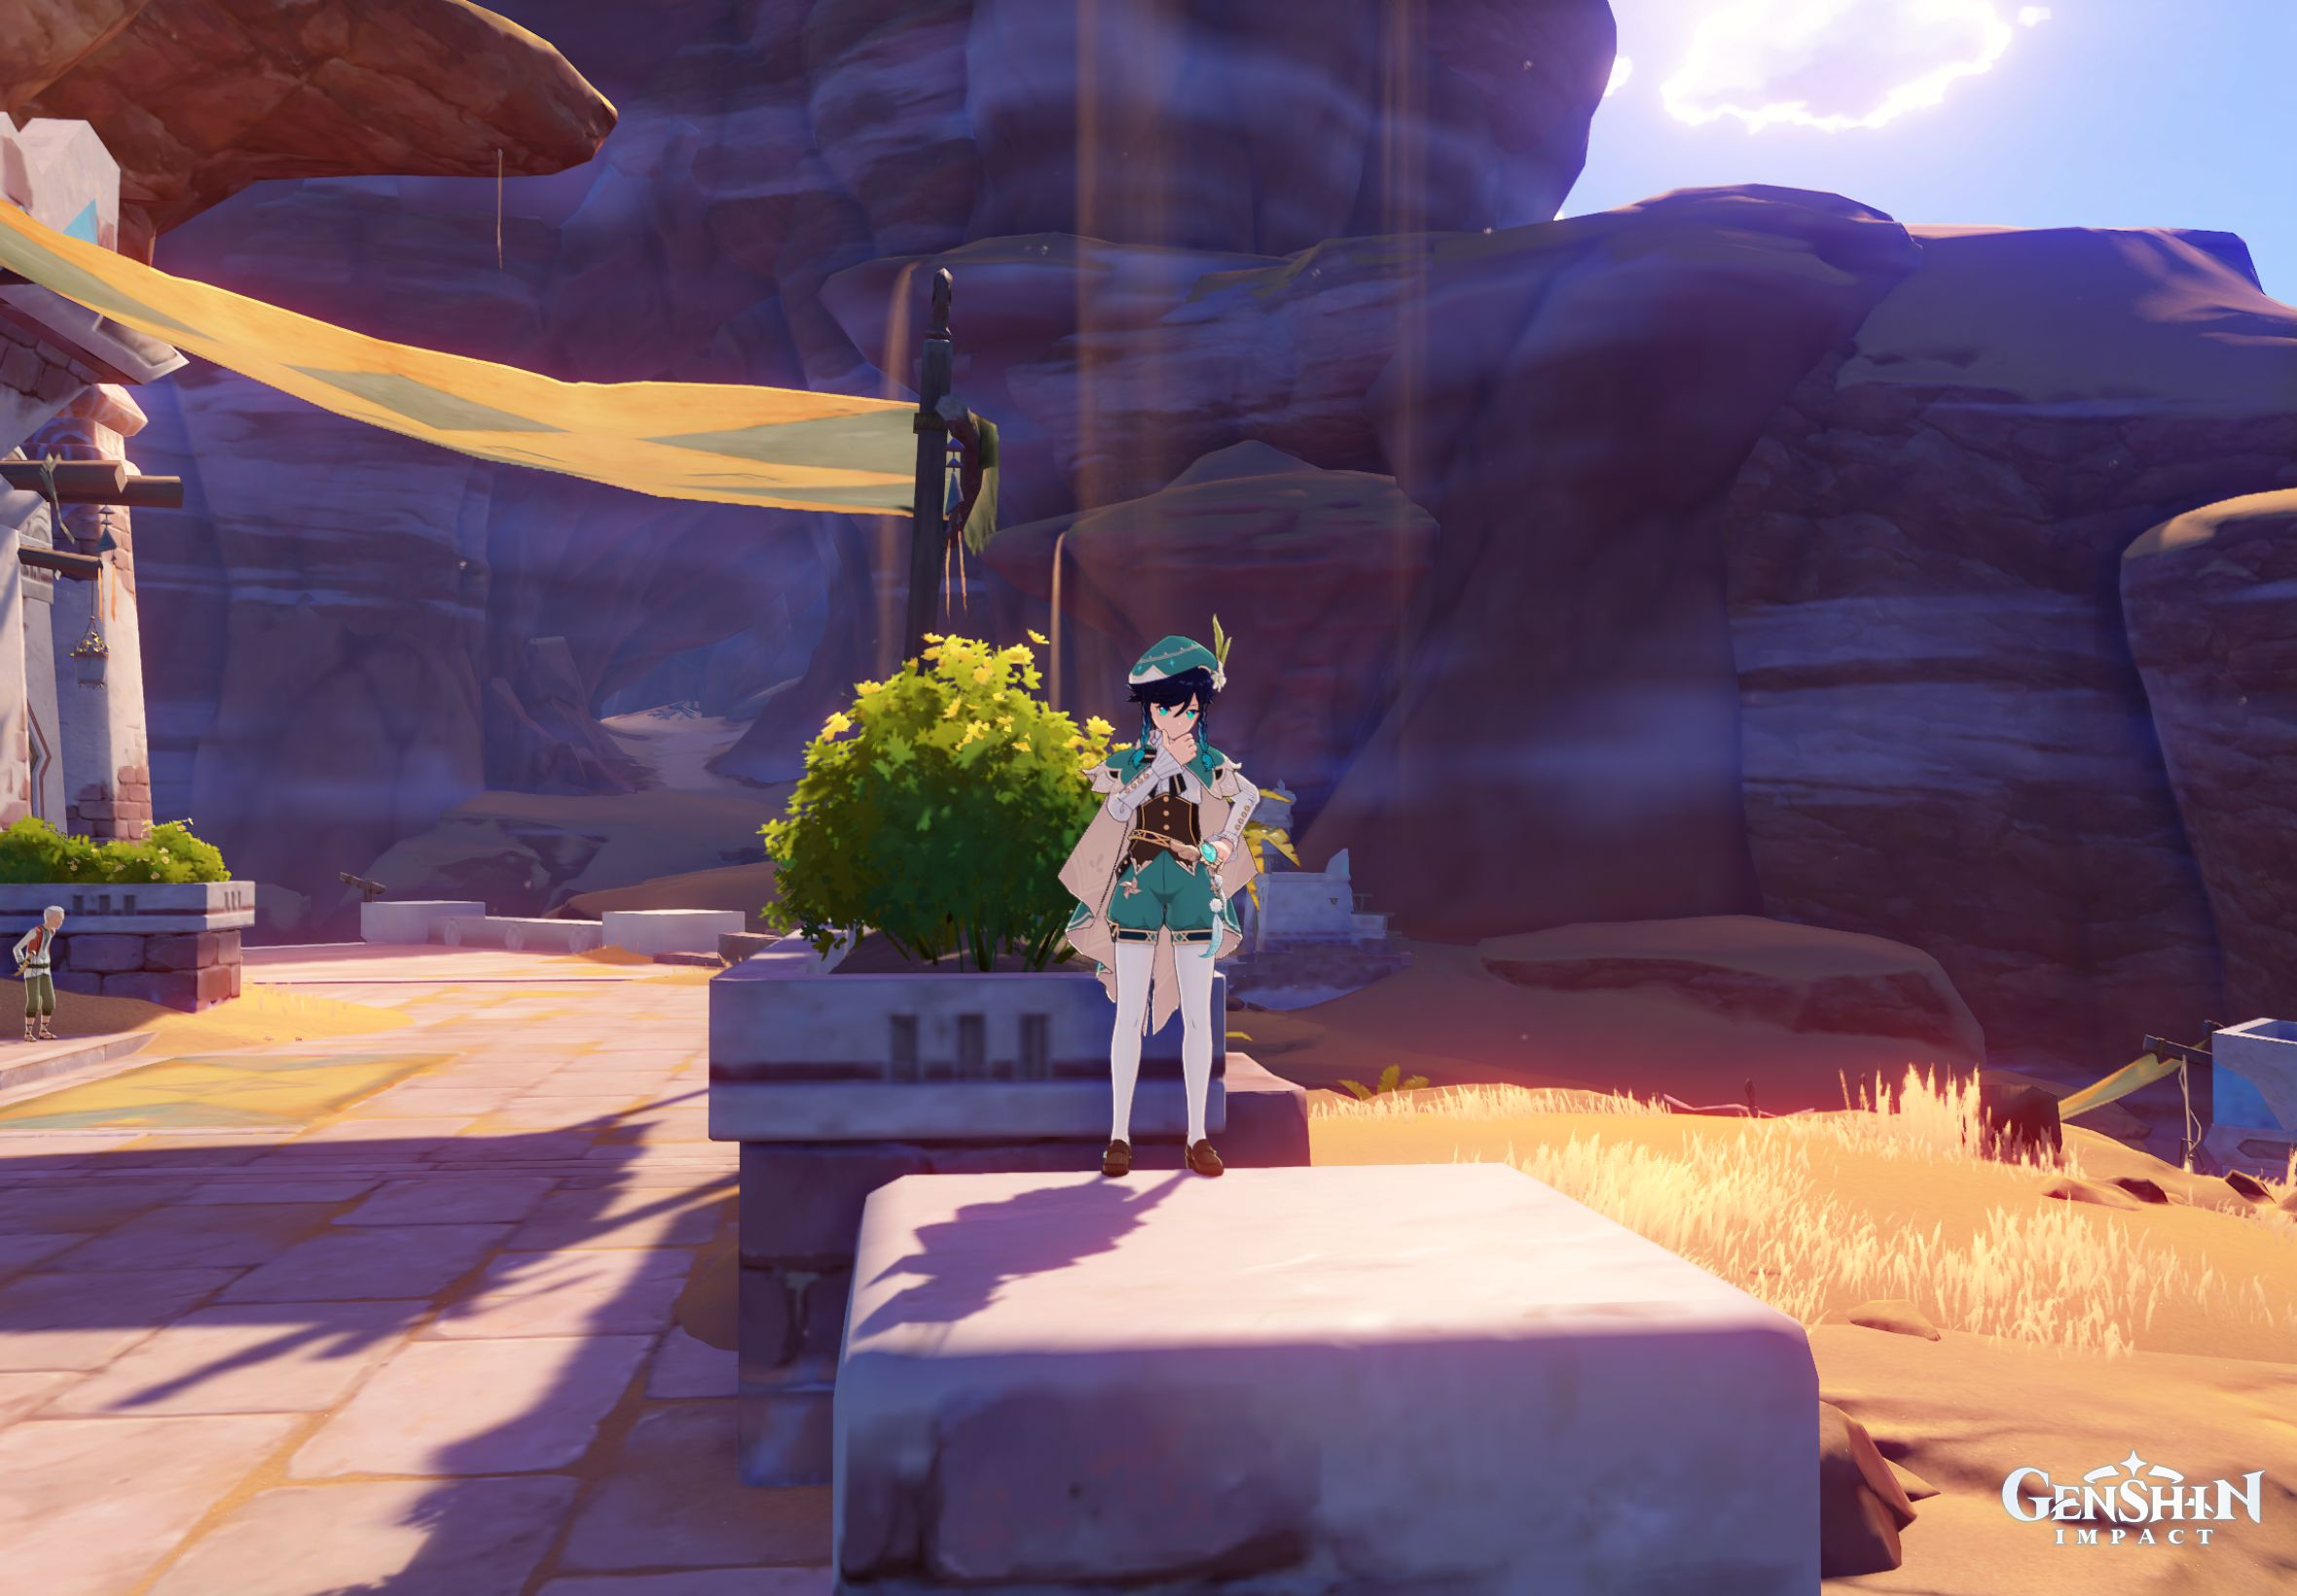
\includegraphics[scale=0.15]{venti.jpg} \\
    \small{Venti is adorable!}
\end{center}